\documentclass[a4paper, 14pt, reqno, oneside]{extbook}

%%%%%%%%%%%%%%%%%%%%%%%%%%%%%%%%%%%%%%%%%%%%%%%%%
% Подключение пакета NeuroFuzzy
%
% Доступные опции:
%    todos       - включить заметки TODO,
%    usebuilddir - указывается при использовании директории build для хранения
%                  временных файлов.
%%%%%%%%%%%%%%%%%%%%%%%%%%%%%%%%%%%%%%%%%%%%%%%%%
\usepackage{NeuroFuzzy}

%%%%%%%%%%%%%%%%%%%%%%%%%%%%%%%%%%%%%%%%%%%%%%%%%
% Файл с библиографией
%%%%%%%%%%%%%%%%%%%%%%%%%%%%%%%%%%%%%%%%%%%%%%%%%
\addbibresource{diploma.bib}

%%%%%%%%%%%%%%%%%%%%%%%%%%%%%%%%%%%%%%%%%%%%%%%%%
% Данные для титульного листа
%
% Типовой вариант:
% 
% \worktype{Дипломная работа}
% \title{Тема диплома}
% \author{студент 435 гр. И.\,О.\;Фамилия}
% \supervisor{к.\,ф.-м.\,н. А.\,В.\;Зубюк}
% \approver{Заведующий каф. математического моделирования и информатики д.\,ф.-м.\,н. проф.}{А.\,И.\;Чуличков}
%%%%%%%%%%%%%%%%%%%%%%%%%%%%%%%%%%%%%%%%%%%%%%%%%
\worktype{Учебно-методическое пособие} % Магистерская диссертация, Дипломная работа, Курсовая работа и т.п.
\title{Пособие для студентов по оформлению курсовых, дипломных и других работ в системе вёрстки научных текстов \LaTeX}
% \author{студент 435 гр. И.\,О.\;Фамилия}
\author{к.\,ф.-м.\,н. доц. кафедры математического моделирования и информатики А.\,В.\;Зубюк}
% \supervisor{к.\,ф.-м.\,н. А.\,В.\;Зубюк} % Научный руководитель: ...
% \approver{Заведующий каф. математического моделирования и информатики д.\,ф.-м.\,н. проф.}{А.\,И.\;Чуличков} % Допущено к защите...
\date{\the\year}

%%%%%%%%%%%%%%%%%%%%%%%%%%%%%%%%%%%%%%%%%%%%%%%%%
% Начало документа
%%%%%%%%%%%%%%%%%%%%%%%%%%%%%%%%%%%%%%%%%%%%%%%%%
\begin{document}

%%%%%%%%%%%%%%%%%%%%%%%%%%%%%%%%%%%%%%%%%%%%%%%%%
% Формирование титульного листа
%%%%%%%%%%%%%%%%%%%%%%%%%%%%%%%%%%%%%%%%%%%%%%%%%
\maketitle

%%%%%%%%%%%%%%%%%%%%%%%%%%%%%%%%%%%%%%%%%%%%%%%%%
% Перечень заметок TODO и оглавление
%%%%%%%%%%%%%%%%%%%%%%%%%%%%%%%%%%%%%%%%%%%%%%%%%
\listoftodos
\tableofcontents

%%%%%%%%%%%%%%%%%%%%%%%%%%%%%%%%%%%%%%%%%%%%%%%%%
% Основное содержание документа
%%%%%%%%%%%%%%%%%%%%%%%%%%%%%%%%%%%%%%%%%%%%%%%%%
\part*{Введение}
\phantomsection\addcontentsline{toc}{part}{Введение}

Как и многие другие научные руководители, я~--- автор этот пособия~--- в какой-то момент осознал, что проще один раз написать краткий <<курс молодого бойца>> по оформлению курсовых и дипломных студенческих работ, чем проводить такой инструктаж персонально для каждого студента, работающего под моим руководством. Результат моих усилий~--- перед вами.

Впрочем, как показывает мой опыт, он может быть полезен и опытным научным работникам, давно работающим с \LaTeX.

В настоящем пособии на примерах показано, как следует оформлять основные элементы курсовой или дипломной работы (титульный лист, разделы, формулы, рисунки, таблицы и \dr) в системе вёрстки научных текстов \LaTeX. О самой системе \LaTeX\xspace рассказано в главе~\ref{sec:about latex}. Основные правила оформления текстов с примерами даются, начиная с главы~\ref{sec:examples}.

Техническая информация о работе с системой \LaTeX\xspace в настоящем пособии перемежается общими рекомендациями по написанию научных текстов, информацией о том, как должна быть структурирована работа, какая информация должна содержаться в тех или иных её разделах.

Студентам предлагается использовать исходный текст настоящего пособия как шаблон своей работы. Его можно скачать с сайта научной группы, руководимой автором пособия, по ссылке\\
\centerline{\uline{\color{blue}\url{http://neurofuzzy.phys.msu.ru/~zubuk/DiplomaTemplate.zip}}.}

Начать изучение предлагается с преобразования скачанного исходного текста в PDF-файл согласно инструкциям, данным в разделах~\ref{sec:simple build}--\ref{sec:texmaker}.
После этого каждый студент, прочитавший настоящее пособие и изучивший его исходный тест, сможет легко преобразовать его под свои нужды. Помогут в этом имеющиеся в исходном тексте пособия комментарии.

Оформление пособия основано на разработанном его автором стилевом файле \texttt{NeuroFuzzy.sty}, который подключается в начале документа:
\begin{minted}{latex}
\usepackage{NeuroFuzzy}
\end{minted}
Оно в основном (но не полностью) соответствует требованиям \href{http://www.viniti.ru/docs/sibid/gost732.pdf}{\color{blue}\uline{ГОСТ~7.32-2017 <<Отчёт о научно-исследовательской работе: структура и правила оформления>>}}.

\chapter{Система вёрстки научных текстов \LaTeX\xspace и её использование}
\label{sec:about latex}

\section{Что такое \LaTeX\xspace и зачем он нужен}

\LaTeX~--- это, пожалуй, самая популярная в мире система вёрстки научных текстов. Все сколь-нибудь значимые научные журналы в области физики и математики оформляются в \LaTeX\xspace (это <<Nature>>, <<Fuzzy Sets and Systems>>, <<Вестник Московского университета>> и многие многие другие), его используют ведущие зарубежные и отечественные издательства научной литературы (например, \href{https://www.elsevier.com/}{{Elsevier}} и \href{http://www.fml.ru/}{{\scshape ФИЗМАТЛИТ}}).

Именно поэтому в нашей научной группе для подготовки курсовых, дипломных и \dr работ мы настоятельно рекомендуем студентам использовать \LaTeX.

Также \LaTeX\xspace удобно использовать для подготовки презентаций. Эта возможность особенно полюбилась математикам из-за удобства вставки формул, поэтому подавляющее большинство презентаций на международных математических конференциях подготовлено в \LaTeX.

Система вёрстки научных текстов \LaTeX\xspace представляет собой совокупность двух компонент:
\begin{enumerate}
\item
    \emph{Специальный язык разметки}. Наверняка вы слышали о языке разметки HTML, используемом для оформления web-страниц. Язык \LaTeX\xspace служит аналогичной цели, но предназначен для оформления научных текстов;
\item
    \emph{Компилятор}, который преобразует исходный текст на языке \LaTeX\xspace (файл с расширением \verb@.tex@), в PDF-файл.
\end{enumerate}

Дистрибутивы компилятора \LaTeX\xspace можно найти для всех основных операционных систем: для Windows можно использовать дистрибутив Mik\TeX, для Linux и \dr Unix-подобных систем~--- \TeX live.

\section{Структура исходных текстов на языке \LaTeX}

Как правило, исходный текст документа состоит из нескольких файлов:
\begin{itemize}
\item
    \emph{Файл с расширением} \verb@.tex@~--- основной файл документа, в котором набран его текст;
\item
    \emph{Файл с расширением} \verb@.bib@~--- файл, в котором в специальном формате Bib\TeX\xspace хранится информация об источниках, на которые в документе даются ссылки (библиография). Сохранять информацию в формате Bib\TeX\xspace умеют все основные библиографические базы: \href{https://scholar.google.com}{\color{blue}\uline{Google Scholar}}, \href{http://webofknowledge.com}{\color{blue}\uline{Web of Science}}, \href{http://scopus.com}{\color{blue}\uline{SCOPUS}} и \dr;
\item
    \emph{Дополнительные файлы}, например, изображения в форматах PDF, JPEG, PNG и \dr или данные для построения графиков. В настоящем шаблоне они хранятся в директории \verb@pictures@.
\end{itemize}

\section{Подготовка (редактирование) исходных текстов на языке \LaTeX}

Исходные тексты на языке \LaTeX~--- это файлы с обычным текстом, их можно создавать и редактировать в любом текстовом редакторе. В Windows это может быть редактор <<Блокнот>> (<<Notepad>>), в Linux и \dr Unix-подобных операционных системах~--- редакторы <<GEdit>>, <<Kate>> и \dr

Однако, наиболее удобно это делать в специальных редакторах, которые умеют <<подсвечивать>> синтаксические конструкции \LaTeX, а также сразу преобразовывать исходные тексты документа в PDF-файл с помощью компилятора \LaTeX. Одним из наиболее популярных редакторов сегодня является \TeX Maker.

\section{Сборка (компиляция) PDF-файла из исходных текстов на языке \LaTeX}
\label{sec:simple build}

В программировании \emph{сборкой} (или \emph{компиляцией}) называют преобразование исходных текстов программы (например, написанных на языке C++) в исполняемый программный модуль (например, в файл с расширение \texttt{.exe}, если речь идёт об операционной системе Windows). В случае работы с \LaTeX\xspace сборкой называют преобразование исходных текстов на языке \LaTeX\xspace в итоговый PDF-файл. Она осуществляется в несколько этапов:
\begin{enumerate}
\item Первый проход утилиты-компилятора \verb@pdflatex@:
\begin{minted}{bash}
pdflatex -shell-escape diploma.tex
\end{minted}
    На этом этапе формируется PDF-файл, однако, этот файл не является окончательным: в нём отсутствуют разделы <<Содержание>> (оглавление) и <<Список использованных источников>>, могут отсутствовать ссылки на некоторые нумерованные объекты (разделы, формулы, рисунки и \dr).
    
    При этом создаются \emph{временные}\footnote{Несмотря на эпитет <<временные>> эти файлы не удаляются автоматически и остаются на диске после завершения сборки.} файлы, в которых сохраняется информация о том, какие номера присвоены разделам, формулам, рисункам и \dr нумерованным объектам документа, о том, на каких страницах они расположены, о том на какие библиографические источники имеются ссылки в документе и \td
    
    Невозможность сразу сформировать окончательный PDF-файл связана с особенностью работы всех компиляторов (в \tch компиляторов программ на языках C/C++ и \dr)~--- при анализе файла с исходными текстами они движутся сверху вниз и никогда не возвращаются обратно. Поэтому одного прохода утилиты-компилятора \texttt{pdflatex} недостаточно для формирования оглавления (\tk неизвестно, на каких страницах окажутся разделы документа), правильных ссылок на нумерованные объекты (\tk ссылка может встретиться в исходном тексте раньше, чем сам нумерованный объект, \te до того, как ему будет присвоен номер) и \td
\item Формирование библиографии утилитой \verb@biber@:
\begin{minted}{bash}
biber diploma
\end{minted}
    На этом этапе на основе собранной ранее информации об использованных библиографических источниках в специальном временном файле формируется исходный текст раздела <<Список использованных источников>>.
\item Второй проход утилиты \verb@pdflatex@:
\begin{minted}{bash}
pdflatex -shell-escape diploma.tex
\end{minted}
    На этом этапе формируется более полный, но всё же ещё не окончательный PDF-файл, в который из сформированных ранее временных файлов вставляется содержимое разделов <<Содержание>>, <<Список использованных источников>>, на места ссылок на нумерованные объекты подставляются номера этих объектов и \td Всей этой информации не было в PDF-файле, сформированном при первом проходе утилиты \verb@pdflatex@. Однако, из-за вставки нового материала некоторые разделы могут оказаться на других страницах в сравнении с PDF-файлом, сформированным при первом проходе утилиты \verb@pdflatex@. В связи с этим номера страниц в разделе <<Содержание>> необходимо обновить, для чего служит следующий шаг.
\item Третий проход утилиты \verb@pdflatex@:
\begin{minted}{bash}
pdflatex -shell-escape diploma.tex
\end{minted}
    На этом этапе формируется итоговый PDF-файл.
\end{enumerate}

\section{Сборка с сохранением временных файлов в отдельной директории}
\label{sec:build dir}

При использовании описанного в предыдущем разделе способа сборки PDF-файла директория с исходными текстами <<замусоривается>> большим количеством временных файлов. Удаление этих файлов после окончания работы с документом~--- достаточно неприятный и трудоёмкий процесс. В связи с этим разумно создать отдельную директорию для хранения временных файлов, например, директорию \verb@build@, и с помощью флага \verb@--output-dir@ <<заставить>> используемые утилиты сохранять все временные файлы в ней. В этом случае сборка PDF-файла может быть осуществлена следующим образом:
\begin{minted}{bash}
mkdir build
pdflatex --output-dir=build -shell-escape diploma.tex
biber --output-dir=build diploma
pdflatex --output-dir=build -shell-escape diploma.tex
pdflatex --output-dir=build -shell-escape diploma.tex
\end{minted}

\begin{notice}
\label{note:usebuilddir}
    При сборке исходных текстов настоящего документа с сохранением временных файлов в директории \verb@build@ необходимо в начале файла \texttt{diploma.tex} при подключении пакета \texttt{NeuroFuzzy} установить опцию \texttt{usebuilddir}:
\begin{minted}{latex}
\usepackage[usebuilddir]{NeuroFuzzy}
\end{minted}
В противном случае сборка приведёт к ошибкам. Это замечание верно и при сборке с использованием редактора \TeX Maker, описанной в разделе~\ref{sec:texmaker}.
\end{notice}

\section{Сборка с использованием утилиты \texttt{make}}
\label{sec:make}

Ещё более удобным способом сборки является использование утилиты \verb@make@ и заранее подготовленного файла \verb@Makefile@, в котором прописаны инструкции по сборке, используемые утилитой \verb@make@. При таком подходе достаточно просто зайти в директорию, где хранятся \verb@Makefile@ и основной файл документа, и выполнить команду
\begin{minted}{bash}
make
\end{minted}
Впрочем, такой способ доступен только пользователям Linux и \dr Unix-подобных операционных систем

\section{Сборка в редакторе \TeX Maker}
\label{sec:texmaker}

Сборку документа удобно осуществлять параллельно с его редактированием в редакторе \TeX Maker. Для этого нужно зайти в редактор и настроить параметры сборки, см. рисунок~\ref{fig:texmaker}. После этого можно выполнять действия, описанные в разделах~\ref{sec:simple build} и~\ref{sec:build dir}, выбирая соответствующие пункты меню <<Tools>>:
\begin{itemize}
\item
    для одного прохода утилиты \texttt{pdflatex} следует выбрать пункт <<Tools~$\to$ PDF\LaTeX>>, <<горячая>> клавиша \texttt{F6};
\item
    для одного прохода утилиты \texttt{biber} следует выбрать пункт <<Tools~$\to$ Bib\TeX>>, <<горячая>> клавиша \texttt{F11}.
\end{itemize}
\begin{figure}
\centerline{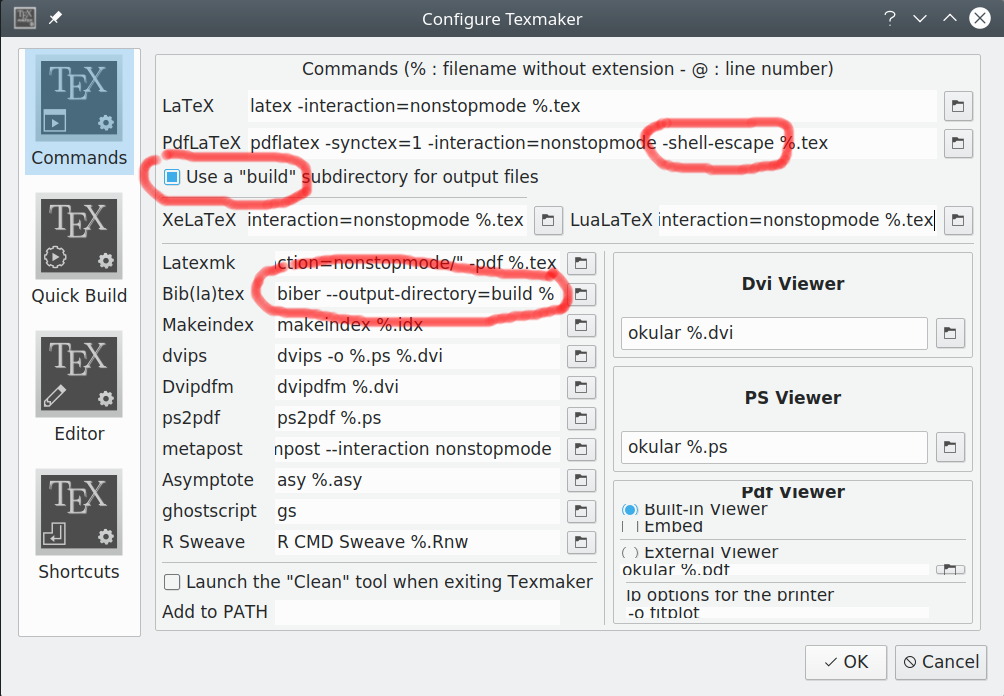
\includegraphics[width=0.9\textwidth]{texmaker-settings}}
\caption{Настройка редактора \TeX Maker (пункт меню <<Options~$\to$ Configure Texmaker>>) для правильной сборки настоящего документа. Обратите внимание на флаг \texttt{-shell-escape} и использование утилиты \texttt{biber} вместо \texttt{bibtex}. Для удобства \TeX Maker настраивается на использование поддиректории \texttt{build} для хранения временных файлов, соответственно, обратите внимание на замечание~\ref{note:usebuilddir}, сделанное выше в разделе~\ref{sec:build dir}.}
\label{fig:texmaker}
\end{figure}

Таким образом, полная сборка результирующего PDF-файла может быть осуществлена следующей последовательность <<горячих>> клавиш:
\centerline{\texttt{F6} $\to$ \texttt{F11} $\to$ \texttt{F6} $\to$ \texttt{F6}.}

Для просмотра результата используйте пункт меню <<Tools~$\to$ View PDF>>, <<горячая>> клавиша \texttt{F7}.
Также удобно использовать <<быструю>> сборку <<Tools~$\to$ Quick Build>>, <<горячая>> клавиша \texttt{F1}.

\chapter{Оформление исходных текстов на языке \LaTeX}
\label{sec:examples}

\section{Набор обычного текста, пробелы, пунктуация}

Исходный текст \LaTeX\xspace в основном файле документа с расширением \verb@.tex@ набирается обычным способом, как это делается в любом текстовом редакторе.

Слова в исходном тексте разделяются пробелами (любым количеством) или переносом строки, при сборке PDF-файла эти символы заменяются на \emph{один} пробел. Таким образом, если при наборе текста вы случайно вставите между словами два или более пробелов, при компиляции <<лишние>> пробелы не будут учтены. Естественно, что использовать множественные пробелы для выравнивания текста в \LaTeX\xspace бессмысленно~--- все они заменятся на одинарный пробел.

Абзацы в исходном тексте отделяются одной или несколькими пустыми строками:
\begin{minted}{latex}
Текст одного абзаца.

Текст другого абзаца.
\end{minted}
Красные строки (отступы в начале абзаца) \LaTeX\xspace проставляет автоматически.

При наборе исходного текста следует обратить внимание на специальные пробелы и знаки пунктуации, используемые в \LaTeX, см. таблицу~\ref{tab:punctuation}. Без их правильного использования итоговый текст в PDF-файле будет выглядеть небрежно.

\begin{table}
\caption{Специальные пробелы и знаки пунктуации в \LaTeX.}
\label{tab:punctuation}
\centering
\begin{tabular}{|C{0.32\textwidth}|C{0.32\textwidth}|C{0.25\textwidth}|}
\hline
\textbf{Описание специального пробела или знака препинания} & \textbf{Пример применения} & \textbf{Специальный символ или команда \LaTeX}\\\hline
Неразрывный пробел переменной длины & таблица~\ref{tab:punctuation} & \verb@~@ \\\hline
Короткий неразрывный пробел & А.\,В.\;Зубюк\par (между А. и В.) & \verb@\,@ \\\hline
Длинный неразрывный пробел & А.\,В.\;Зубюк\par (между инициалами и фамилией) & \verb@\;@ \\\hline
Дефис\par (короткая черта) & физ.-мат. науки & \verb@-@ \\\hline
Минус (средняя черта) & стр.~1--10 & \verb@--@ \\\hline
Тире (длинная черта) & Тире~--- длинная черта\par (между знаком тире и предшествующим словом рекомендуется ставить неразрывный пробел \verb@~@, чтобы тире не переносилось на другую строку или страницу) & \verb@---@ \\\hline
Русские кавычки-<<ёлочки>> & Метро <<Университет>> & \verb@<<@ (откр.)\par \verb@>>@ (закр.) \\\hline
Английские кавычки-<<лапки>> & Next stop is ``University'' & \verb@``@ и \verb@''@\par (см. буквы <<ё>>~и~<<э>> на клавиатуре) \\\hline
\end{tabular}
\end{table}

Неразрывные пробелы следует вставлять между словами, которые не должны разделяться переносом строки или переходом на другую страницу. Например, между словом <<таблица>> и номером таблицы~\ref{tab:punctuation} в ссылке неё. При этом различают неразрывные пробелы переменной и фиксированной длины. Первые имеют ту же длину, которую имеют все пробелы в данной строке (длины пробелов в разных строках различаются, за счёт этого текст выравнивается по ширине страницы). Вторые имеют фиксированную длину. Типовые примеры применения неразрывных пробелов даны в таблице~\ref{tab:punctuation}.

К специальным знакам пунктуации отнесём разные виды черт, применяющиеся в разных синтаксических конструкциях: дефис, минус и тире. Также к ним отнесём кавычки. Для их набора в \LaTeX\xspace используются специальные сочетания символов. Типовые примеры их применения даны в таблице~\ref{tab:punctuation}.

\section{Разделы, формулы, их нумерация и ссылки на них}
\label{sec:sections}

Заголовки разделов в \LaTeX\xspace создаются командами (макросами) \mintinline{latex}{\part}, \mintinline{latex}{\chapter}, \mintinline{latex}{\section}, \mintinline{latex}{\subsection} и \td Все разделы нумеруются автоматически. Для того, чтобы сослаться на раздел, после команды, формирующей его заголовок, необходимо вставить \emph{метку} с помощью команды \mintinline{latex}{\label{метка}}, где \mintinline{latex}{метка}~--- придуманный вами уникальный идентификатор раздела, по которому на него можно будет ссылаться. Например, настоящий раздел~\ref{sec:sections} на стр.~\pageref{sec:sections} под названием <<\nameref{sec:sections}>> в исходном тексте начинается так:
\begin{minted}{latex}
\section{Разделы, формулы, их нумерация и ссылки на них}
\label{sec:sections}
\end{minted}
Для ссылок на него использованы команды \mintinline{latex}{\ref{sec:sections}} (номер раздела), \mintinline{latex}{\pageref{sec:sections}} (страница, где начинается раздел) и \mintinline{latex}{\nameref{sec:sections}} (текст заголовка).

Аналогично (с помощью команд \mintinline{latex}{\label}, \mintinline{latex}{\ref}, \mintinline{latex}{\pageref}) оформляются ссылки на любые другие нумерованные объекты: таблицы, рисунки и \tp Ссылки на формулы создаются с помощью команды \mintinline{latex}{\eqref}, которая заключает номер формулы в круглые скобки, как это принято в научной литературе.

Формулы бывают \emph{обособленными} (на отдельной строке) и \emph{встроенными} (внутри обычного текста). Обособленные формулы могут нумероваться, а могут~--- нет. Для создания встроенных формул используются знаки доллара: \mintinline{latex}{$формула$}. Для создания нумерованных формул следует использовать окружения \mintinline{latex}{equation}, \mintinline{latex}{multline}, \mintinline{latex}{gather}, \mintinline{latex}{align} и \dr, например:
\begin{minted}{latex}
\begin{equation}
    формула
\end{equation}
\end{minted}
Нумеровать следует только те формулы, на которые в тексте есть ссылки. Например, формула~\eqref{eq:circle} позволяет связать площадь круга $S$ с его радиусом~$r$:
\begin{equation}
\label{eq:circle}
    S = \pi r^2.
\end{equation}
А вот выражение для длины окружности~$l$:
\[
    l = 2\pi r.
\]
На него в тексте нет ссылки, поэтому использованы скобки \mintinline{latex}{\[} и \mintinline{latex}{\]} для создания ненумерованной обособленной формулы. Также ненумерованные формулы можно создавать с помощью окружений <<со звёздочкой>>: \mintinline{latex}{equation*}, \mintinline{latex}{multline*}, \mintinline{latex}{gather*}, \mintinline{latex}{align*} и \dr

Внутри формул вы можете использовать всевозможные специальные знаки: индексы, греческие буквы, интегралы и \td Для их набора следует использовать специальные команды и символы \LaTeX:
\begin{itemize}
\item
    нижние и верхние индексы: \mintinline{latex}{a^i, a_j, A^i_j}
    \[a^i,\ a_j,\ A^i_j;\]
\item
    греческие буквы: \mintinline{latex}{\alpha, \beta, \gamma, \Gamma, \omega, \Omega} и \dr
    \[\alpha,\ \beta,\ \gamma,\ \Gamma,\ \omega,\ \Omega;\]
\item
    интегралы: \mintinline{latex}{\int\limits_{0}^\infty, \iint, \oint} и \dr
    \[\int\limits_{0}^\infty,\ \iint,\ \oint;\]
\item
    сумма \mintinline{latex}{\sum_{i=1}^n} и произведение \mintinline{latex}{\prod_{i=1}^n}
    \[\sum_{i=1}^n,\ \prod_{i=1}^n;\]
\item
    дроби: \mintinline{latex}{\frac{a}{b}, \dfrac{a}{b}}
    \[\tst\frac{a}{b},\ \dfrac{a}{b};\]
\item
    символы математических функций, операторов и отношений: \mintinline{latex}{\sin, \exp, \partial, \nabla, \sim, \approx, \in, \subset, \notin, \min_a, \max_a, \inf_a, \sup_a, \lim_{a\to b}} и \dr
    \[\sin,\ \exp,\ \partial,\ \nabla,\ \sim,\ \approx,\ \in,\ \subset,\ \notin,\ \min_a,\ \max_a,\ \inf_a,\ \sup_a,\ \lim_{a\to b};\]
\item
    векторы и другое декорирование: \mintinline{latex}{\vec a, \tilde a, \hat a, \widetilde{abc}} и \dr
    \[\vec a,\ \tilde a,\ \hat a,\ \widetilde{abc};\]
\item
    матрицы: \mint{latex}@\begin{pmatrix}1 & 2 & 3\\ 4 & 5 & 6\end{pmatrix}@
    \[\begin{pmatrix}1 & 2 & 3\\ 4 & 5 & 6\end{pmatrix};\]
\item
    стрелки: \mintinline{latex}{\xrightarrow[n\to\infty]{\text{п.\,н.}}, \to, \Rightarrow, \Leftarrow}
    \[\xrightarrow[n\to\infty]{\text{п.\,н.}},\ \to,\ \Rightarrow,\ \Leftarrow;\]
\item
    многострочные формулы, системы уравнений, скобки
    \begin{minted}{latex}
\begin{gather*}
    S = \pi r^2,\ l = 2\pi r,\\
    |a| = \begin{cases}a, & a>0,\\-a, &a\leqs 0,\end{cases}\\
    \left\{ \int\limits_{-\infty}^\infty  f(x, c) dx \;\middle|\; c\in [0,1] \right\}.
\end{gather*}
    \end{minted}
    \begin{gather*}
        S = \pi r^2,\ l = 2\pi r,\\
        |a| = \begin{cases}a, & a>0,\\-a, &a\leqs 0,\end{cases}\\
        \left\{ \int\limits_{-\infty}^\infty  f(x, c) dx \;\middle|\; c\in [0,1] \right\}.
    \end{gather*}
\end{itemize}

\section{Оформление рисунков и таблиц}

Рисунки и таблицы принято считать <<плавающими>> объектами. Это означает, что они могут располагаться в тексте не там, где даётся их описание. Так, например, согласно ГОСТ рисунок может располагаться на той странице, где даётся его описание (точнее~--- ссылка на него), или же на следующей странице. Иногда все рисунки и таблицы печатают к конце документа.

\LaTeX\xspace автоматически выбирает наиболее подходящее расположение для рисунков и таблиц. Без крайней необходимости не ст\'{о}ит вмешиваться в этот механизм и пытаться <<заставить>> рисунок или таблицу расположиться в каком-то ином месте.

Важно помнить, что каждый рисунок и каждая таблица должны быть подписаны, \te должны иметь заголовок. Заголовки создаются с помощью команды \mintinline{latex}{\caption}, которая сама печатает постоянную часть заголовка (слово <<Рисунок>> или <<Таблица>>), проставляет очередной номер, печатает символ-разделитель (тире).
Также важно помнить, что на каждый рисунок и каждую таблицу в основном тексте документа \emph{обязательно} должна быть ссылка, сделанная с помощью команды \mintinline{latex}{\label}.

Пример таблицы был дан выше, см. таблицу~\ref{tab:punctuation}, как и пример обычного рисунка (\te рисунка, который состоит из изображения, вставленного из графического файла), см. рисунок~\ref{fig:texmaker}.

В общем-то, любой рисунок можно оформить простой вставкой изображения из графического файла. Однако, в научных работах мы очень часто имеем дело с графиками, построенными по данным физического эксперимента, расчётов и \tp Для построения таких графиков лучше использовать средства самого \LaTeX, \tk это позволит оформить все графики в работе в едином стиле (одинаковые толщины линий, шрифты подписей и \td), согласованном со стилем основного текста (размеры шрифтов, начертание символов, в \tch греческих букв, и \tp).

При использовании <<внешних>> программ для подготовки графиков соблюсти единообразие оформления не удастся, и графики будут выглядеть небрежно. Кроме того, графики, оформленные средствами \LaTeX, легко переносятся из исходных текстов, предназначенных для печати на бумаге в формате A4, в презентации (конечно же, речь идёт о презентациях, сделанных в \LaTeX), \tk при сборке PDF-файла презентации оформление графиков автоматически будет приведено к стилю презентации. При использовании <<внешних>> программ графики для презентаций придётся делать заново, \tk подписи графиков в презентациях принято делать \emph{значительно} крупнее, чем в печатных текстах (иначе их просто не будет видно слушателям).

Для построения графиков средствами \LaTeX\xspace данные, по которым строятся графики, следует сохранить в форме таблицы в обычный текстовый файл и использовать средства пакета \texttt{tikz} и окружения \mintinline{latex}{\begin{tikzpicture}...\end{tikzpicture}}, см. рисунок~\ref{fig:identification-a}, построенный по данным из файла \texttt{pictures/identification.dat}. На рисунке~\ref{fig:possibility} показано, как строить <<столбиковые>> гистограммы и делать легенды на графиках.

\begin{figure}
\subfigure[Зависимость средней частоты ошибок идентификации от отношения <<шум/сигнал>> корня из дисперсии аддитивного шума, искажающего предъявленные изображения, к разности максимальной и минимальной яркостей неискажённых изображений.]{%
\label{fig:identification-a}
\begin{tikzpicture}
\begin{axis}[
    width=0.5\textwidth, height=0.4\textwidth,
    xlabel={отношение <<шум/сигнал>>}, ylabel={средняя частота ошибок},
    ymin=-0.002, ymax=1, xmode=log
]
\addplot[blue] table[x=sigma, y=alpha] {pictures/identification.dat};
\end{axis}
\end{tikzpicture}}
\hfill
\begin{minipage}{0.45\textwidth}
\mbox{}\\[-2.7cm]
\subfigure[Изображения цифр <<0>>--<<9>>, не искажённые шумом.]{%
\begin{minipage}{\textwidth}

\includegraphics[width=0.19\textwidth, frame]{digits/0}\hfill

\includegraphics[width=0.19\textwidth, frame]{digits/1}\hfill

\includegraphics[width=0.19\textwidth, frame]{digits/2}\hfill
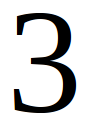
\includegraphics[width=0.19\textwidth, frame]{digits/3}\hfill

\includegraphics[width=0.19\textwidth, frame]{digits/4}\\
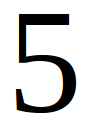
\includegraphics[width=0.19\textwidth, frame]{digits/5}\hfill
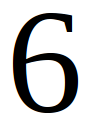
\includegraphics[width=0.19\textwidth, frame]{digits/6}\hfill

\includegraphics[width=0.19\textwidth, frame]{digits/7}\hfill

\includegraphics[width=0.19\textwidth, frame]{digits/8}\hfill

\includegraphics[width=0.19\textwidth, frame]{digits/9}\\[-2mm]
\end{minipage}}
\subfigure[Изображения цифры <<5>>, демонстрирующие интенсивность шума при отношении <<шум/сигнал>>, равном 0.1, 1 и 10.]{%
\begin{minipage}{\textwidth}
\centerline{%
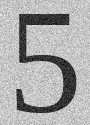
\includegraphics[width=0.19\textwidth]{digits/5-sigma0p1}\;
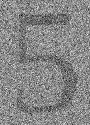
\includegraphics[width=0.19\textwidth]{digits/5-sigma1p0}\;

\includegraphics[width=0.19\textwidth]{digits/5-sigma10p0}}
\mbox{}\\[-8mm]
\end{minipage}}
\end{minipage}
\caption{Иллюстрация работы морфологического алгоритма идентификации печатных цифр <<0>>--<<9>>, искажённых случайным аддитивным шумом.}
\label{fig:identification}
\end{figure}

\begin{figure}
\centering
\begin{tikzpicture}
\begin{axis}[
    width = 0.37\textwidth, height = 0.32\textwidth,
    ymin = 0, ymax = 1.1,
    xtick = {1, 2, 3, 4, 5},
    xticklabels = {$V_1$, $V_2$, $V_3$, $V_4$, $V_5$},
    xmin = 0.4, xmax = 5.6,
    ybar, bar width = 3mm,
    legend style = {at = {(0.5,0.98)}, anchor=north}
]
\addplot[blue, thick, pattern=north east lines, pattern color=blue] table[x=omega, y=p1] {pictures/experiments-1-new-distr.txt};
\addplot[red!80!black, fill=red!80!black] table[x=omega, y=p2] {pictures/experiments-1-new-distr.txt};
\legend{\textcolor{blue}{\small $\pi_1(\cdot)$}, \textcolor{red!80!black}{\small $\pi_2(\cdot)$}}
\end{axis}
\end{tikzpicture}%
\hfill%
\begin{tikzpicture}
\begin{axis}[
    width = 0.37\textwidth, height = 0.32\textwidth,
    ymin = 0, ymax = 1.1,
    xtick = {1, 2, 3, 4, 5},
    xticklabels = {$V_1$, $V_2$, $V_3$, $V_4$, $V_5$},
    xmin = 0.4, xmax = 5.6,
    ybar, bar width = 3mm,
    legend style = {at = {(0.5,0.98)}, anchor=north}
]
\addplot[blue, thick, pattern=north east lines, pattern color=blue] table[x=omega, y=pr1_1] {pictures/experiments-1-new-distr.txt};
\addplot[red!80!black, fill=red!80!black] table[x=omega, y=pr1_2] {pictures/experiments-1-new-distr.txt};
\legend{\textcolor{blue}{\small $p^{(1)}_1(\cdot)$}, \textcolor{red!80!black}{\small $p^{(2)}_1(\cdot)$}}
\end{axis}
\end{tikzpicture}%
\hfill%
\begin{tikzpicture}
\begin{axis}[
    width = 0.37\textwidth, height = 0.32\textwidth,
    ymin = 0, ymax = 1.1,
    xtick = {1, 2, 3, 4, 5},
    xticklabels = {$V_1$, $V_2$, $V_3$, $V_4$, $V_5$},
    xmin = 0.4, xmax = 5.6,
    ybar, bar width = 3mm,
    legend style = {at = {(0.5,0.98)}, anchor=north}
]
\addplot[blue, thick, pattern=north east lines, pattern color=blue] table[x=omega, y=pr2_1] {pictures/experiments-1-new-distr.txt};
\addplot[red!80!black, fill=red!80!black] table[x=omega, y=pr2_2] {pictures/experiments-1-new-distr.txt};
\legend{\textcolor{blue}{\small $p^{(1)}_2(\cdot)$}, \textcolor{red!80!black}{\small $p^{(2)}_2(\cdot)$}}
\end{axis}
\end{tikzpicture}

\caption{Распределения $\pi_i(\cdot)$ и $p^{(i)}_l(\cdot)$ возможностей $\Pi_i$ и вероятностей $P^{(i)}_l,\ {i,\, l=1,\, 2}$, определяющих возможностные модели ${(\mathbf{V},\, \mathcal{A},\, \Pi_1)},\ {(\mathbf{V},\, \mathcal{A},\, \Pi_2)}$ случайных форм изображений, максимально согласованные в совокупности как с вероятностными моделями ${\big(\mathbf{V},\, \mathcal{A},\, P^{(1)}_1\big)},\ {\big(\mathbf{V},\, \mathcal{A},\, P^{(2)}_1\big)}$, так и с ${\big(\mathbf{V},\, \mathcal{A},\, P^{(1)}_2\big)},\ {\big(\mathbf{V},\, \mathcal{A},\, P^{(2)}_2\big)}$. Здесь $\mathbf{V} = \{V_1,\, \ldots,\, V_5\}$, $\mathcal{A}=2^\mathbf{V}$.}
\label{fig:possibility}
\end{figure}

\section{Ускорение набора исходных текстов с помощью определения собственных команд (макросов)}

Набор исходных текстов можно \emph{кардинально ускорить}, если для часто повторяющихся фрагментов (например, сложных математических обозначений, встречающихся во многих формулах документа) определить собственные команды (макросы). Например, вместо того, чтобы везде в тексте набирать громоздкую конструкцию
\begin{minted}{latex}
F_\text{\rm LDR}
\end{minted}
можно определить краткую команду \mintinline{latex}{\FLDR}:
\begin{minted}{latex}
\newcommand{\FLDR}{F_\text{\rm LDR}}
\end{minted}
и далее везде в тексте использовать её.

\newcommand{\FLDR}{F_\text{\rm LDR}}

Как правило, определение собственных команд производят в \emph{преамбуле} документа, \te до строки
\begin{minted}{latex}
\begin{document}
\end{minted}
Но это не является обязательным требованием.

\section{Набор теорем, лемм, следствий, доказательств, определений, примеров и замечаний}

Для набора теорем, лемм, следствий, доказательств, определений, примеров и замечаний в пакете \texttt{NeuroFuzzy} определены окружения \texttt{theorem}, \texttt{lemm}, \texttt{conseq}, \texttt{proof}, \texttt{definition}, \texttt{example} и \texttt{notice} соответственно. Их использование имеет следующий вид:
\begin{minted}{latex}
\begin{theorem}
    Текст теоремы.
\end{theorem}
\begin{proof}
    Доказательство
\end{proof}
\end{minted}

В качестве примера см. теорему~\ref{th:theorem}.
\begin{theorem}
\label{th:theorem}
    $\FLDR(\pi) \subset F_*(\pi)$.
\end{theorem}
\begin{proof}
Assume that $f\in\FLDR(\pi)$ but $f\notin F_*(\pi)$. Then $\exists g\in F$ such that $\max \big\{\pi(s) \,\big|$ $u(g(s)) \ne u_{\max}(s) \big\} < \max \big\{\pi(s) \,\big|\, u(f(s)) \ne u_{\max}(s) \big\}$. Therefore, there exists integer $i$ s.\,t. $u(g(s)) = u_{\max}(s),\ \forall s\in S_1^\pi\cup\ldots\cup S_i^\pi$, while $u(f(s_0)) < u_{\max}(s_0) = u(g(s_0))$ for some $s_0\in S_i^\pi$. Thus, $g >_\pi f$ which contradicts to the initial assumption.
\end{proof}

\section{Оформление списка литературы и ссылок на литературу}

Согласно ГОСТ ссылки на литературу даются в квадратных скобках, см.~ниже, при этом источники нумеруются в том порядке, в котором они встречаются в основном тексте. Т.\,е. первый встретившийся источник должен иметь номер~1, второй~--- номер~2 и \td Это противоречит здравому смыслу и правилам, принятым в большинстве международных научных журналов, \tk делает практически неразрешимой задачу поиска нужного источника (например, когда вам известен автор статьи, и вы хотите найти эту статью) в объёмном списке источников. Но таковы требования ГОСТ.

Ниже в настоящем разделе приведён текст, изобилующий ссылками на литературу, которые будут полезны студентам кафедры математического моделирования и информатики.

Современную аксиоматику теории вероятностей впервые предложил отечественный учёный А.\,Н.\;Колмогоров в своей работе~\cite{cit:kolmogorov}. А вот ещё несколько <<классических>> книг по теории вероятностей: \cite{cit:feller, cit:neveu, cit:shir, cit:probbook-2010}. Вот несколько хороших книг по математической статистике: \cite{cit:leman, cit:barra, cit:borovkov-1997}. О теории нечётких множеств Л.\;Заде и направлениях теории возможностей, развиваемых иностранными авторами, поведают замечательные работы~\cite{cit:Zadeh-1978, cit:dubois_prade-1990}, а о теории возможностей, развиваемой на кафедре математического  моделирования и информатики,~--- работы~\cite{cit:possbook-2000, cit:possbook-2007}. Чтобы узнать о морфологическом анализе изображений Ю.\,П.\;Пытьева, см.~\cite{cit:PytyevMorphI, cit:PytyevMorphII, cit:PytyevMorphIII, cit:morph_book, cit:VizilterTh, cit:vizilter_lectures}.

\part*{Заключение}
\phantomsection\addcontentsline{toc}{part}{Заключение}

В заключении подытоживаются результаты исследования. Делается акцент на основных идеях и результатах работы, изложенных в основной части. Указывается, в каких областях науки и техники и при каких условиях эти идеи и результаты могут быть полезны. Делаются предположения о том, как можно было бы продолжить и развить проведённые исследования.

\part*{Список использованных источников}
\phantomsection\addcontentsline{toc}{part}{Список использованных источников}
\printbibliography[heading=none]

\appendix

\chapter{Зачем нужны приложения}

В приложения выносится материал, который не имеет принципиального значения для понимания основного текста. Приложения можно разбивать на разделы с помощью команд \mintinline{latex}{\section}, \mintinline{latex}{\subsection} и \td, как и обычные главы. Ссылки на приложения делаются точно так же, как и на любые другие разделы.

Приложения создают только в том случае, если в этом есть необходимость. Очень часто приложений в курсовых, дипломных и \dr работах нет, в этом случае работа оканчивается разделом <<Список использованных источников>>.

\chapter{Справочник часто используемых специальных символов и команд \LaTeX}

\begin{longtable}{|C{0.32\textwidth}|C{0.32\textwidth}|C{0.32\textwidth}|}
\caption{Часто используемые специальные символы и команды.}\\\hline
\textbf{Пример} & \textbf{Исходный текст} & \textbf{Описание}\\\hline
\endfirsthead
\caption{продолжение.}\\\hline
\textbf{Пример} & \textbf{Исходный текст} & \textbf{Описание}\\\hline
\endhead
%%%%%
\multicolumn{3}{c}{}\\
\multicolumn{3}{c}{\textit{Пробелы и пунктуация}}\\\hline
таблица~1 & \mintinline{latex}{таблица~1} & неразрывный пробел переменной длины\\\hline
А.\,В.\;Зубюк & \mintinline{latex}{А.\,В.\;Зубюк} & короткий и длинный неразрывные пробелы\\\hline
физ.-мат. науки & \mintinline{latex}{физ.-мат. науки} & дефис\\\hline
стр.~1--10 & \mintinline{latex}{стр.~1--10} & минус или диапазон\\\hline
тире~--- длинная черта & \mintinline{latex}{тире~--- длинная черта} & тире\\\hline
метро <<Университет>> & \mintinline{latex}{метро <<Университет>>} & кавычки-<<ёлочки>>\\\hline
next stop is ``University'' & \mintinline{latex}{next stop is ``University''} & кавычки-<<лапки>>\\\hline
%%%%%
\multicolumn{3}{c}{}\\
\multicolumn{3}{c}{\textit{Метки и ссылки}}\\\hline
& \mintinline{latex}{\label{sec:make}} & метка\\\hline
раздел~\ref{sec:make} & \mintinline{latex}{раздел~\ref{sec:make}} & ссылка по номеру\\\hline
стр.~\pageref{sec:make} & \mintinline{latex}{стр.~\pageref{sec:make}} & ссылка на страницу\\\hline
раздел <<\nameref{sec:make}>> & \mintinline{latex}{раздел <<\nameref{sec:make}>>} & ссылка на заголовок\\\hline
\eqref{eq:circle} & \mintinline{latex}{\eqref{eq:circle}} & ссылка на формулу\\\hline
%%%%%
\multicolumn{3}{c}{}\\
\multicolumn{3}{c}{\textit{Математика}}\\\hline
$a^i, a_j, A^i_j$ & \mintinline{latex}{a^i, a_j, A^i_j} & индексы\\\hline
$\alpha, \beta, \Omega$ & \mintinline{latex}{$\alpha, \beta, \Omega$} & греческие буквы\\\hline
$\int\limits_{0}^\infty, \iint, \oint$ & \mintinline{latex}{$\int\limits_{0}^\infty, \iint, \oint$} & интегралы\\\hline
$\dst\sum_{i=1}^n$ & \mintinline{latex}{$\sum_{i=1}^n$} & сумма\\\hline
$\dst\prod_{i=1}^n$ & \mintinline{latex}{$\prod_{i=1}^n$} & произведение\\\hline
$\frac{a}{b}, \dfrac{a}{b}$ & \mintinline{latex}{$\frac{a}{b}, \dfrac{a}{b}$} & дроби\\\hline
$\sin, \exp, \partial, \nabla, \sim, \approx, \in,$ $\subset, \notin, \dst\min_a, \max_a, \inf_a, \sup_a,$ $\dst\lim_{a\to b}$ & \mintinline{latex}{$\sin, \exp, \partial, \nabla, \sim, \approx, \in, \subset, \notin, \min_a, \max_a, \inf_a, \sup_a, \lim_{a\to b}$} & математические функции, операторы и отношения\\\hline
$\vec a, \tilde a, \hat a, \widetilde{abc}$ & \mintinline{latex}{$\vec a, \tilde a,}\par \mintinline{latex}{\hat a, \widetilde{abc}$} & векторы и другое декорирование\\\hline
$\begin{pmatrix}1 & 2 & 3\\ 4 & 5 & 6\end{pmatrix}$ & \mintinline{latex}{$\begin{pmatrix} 1 & 2 & 3\\ 4 & 5 & 6 \end{pmatrix}$} & матрица\\\hline
$\xrightarrow[n\to\infty]{\text{п.\,н.}}, \to, \Rightarrow, \Leftarrow$ & \mintinline{latex}{$\xrightarrow [n\to\infty] {\text{п.\,н.}}, \to, \Rightarrow, \Leftarrow$} & стрелки,\par текст в формуле\\\hline
$|a|, \|a\|, \left(1 + \dfrac{a}{b}\right)$ & \mintinline{latex}{$|a|, \|a\|, \left(1 + \frac{a}{b}\right)$} & модуль, норма, большие скобки\\\hline
$x=0$\hspace{0.1\textwidth} & \mintinline{latex}{\[ x=0 \]} & обособленная формула\\\hline
$x=0$\hspace{0.1\textwidth}(1) & \mintinline{latex}{\begin{equation} x=0 \end{equation}} & нумерованная формула\\\hline
$\delta_{ij} = \begin{cases} 0\\ 1 \end{cases}$ & \mintinline{latex}{$\delta_{ij} = \begin{cases} 0\\ 1 \end{cases}$} & варианты, система уравнений\\\hline
$S = \pi r^2,$\par $l = 2\pi r.$ & \mintinline{latex}{\begin{gather*} S = \pi r^2,\\ l = 2\pi r. \end{gather*}} & объединение формул\\\hline
$S = \pi r^2 =$\hspace{20mm}\;\par \hspace{20mm}$= \pi d^2/4$ & \mintinline{latex}{\begin{multline*} S = \pi r^2 =\\ = \pi d^2/4 \end{multline*}} & многострочная формула\\\hline
\end{longtable}

\end{document}
